\chapter[dsPICDEM 1.1 Plus Board]{dsPICDEM 1.1 Plus Board}

\section{Introduction}

This chapter describes the support done in \ee\ for the
Microchip dsPICDEM 1.1 Plus Board (see Figure \ref{fig:dspicdem}).

\begin{figure}
  \begin{center}
    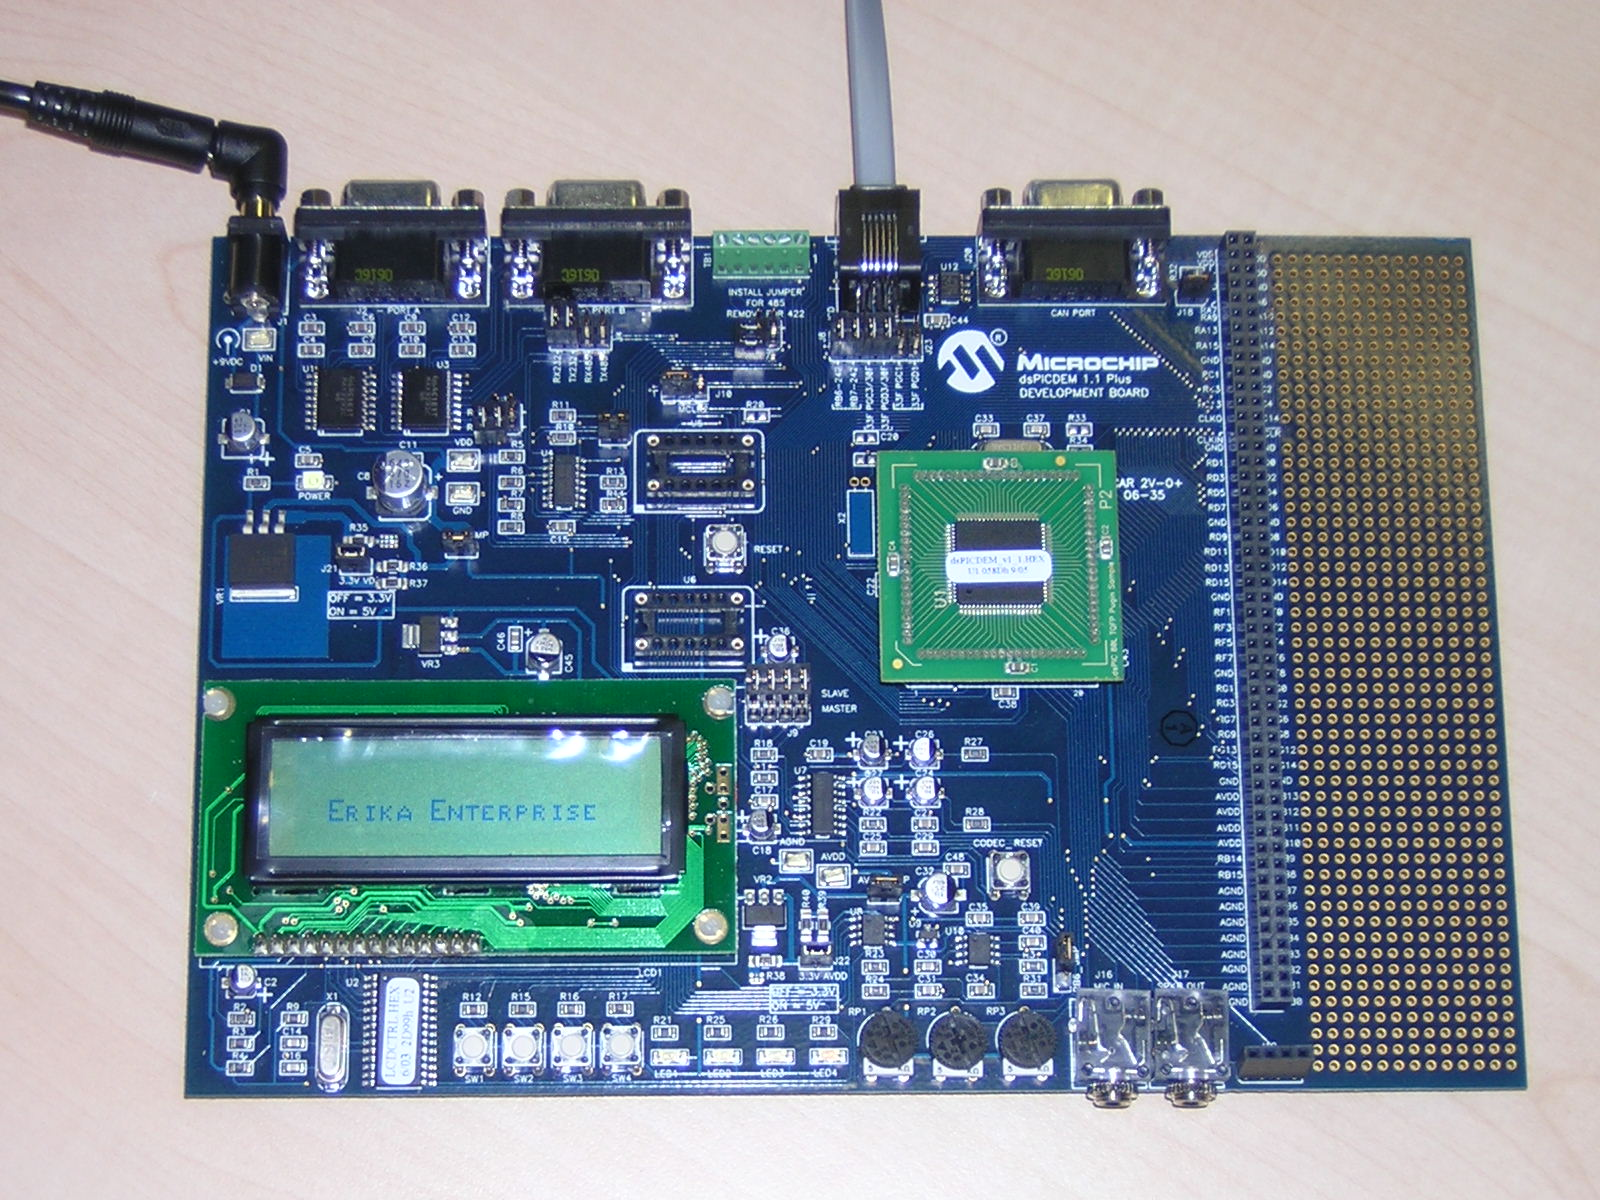
\includegraphics[width=10cm, bb=0 0 1600 1200]{images/dspicdemrunning.jpg}
  \end{center}
  \caption{The Microchip dsPICDEM 1.1 Plus board running \ee.}
  \label{fig:dspicdem}
\end{figure}

The dsPICDEM 1.1 Plus is a low cost, efficient development board
produced by Microchip hosting a graphic display, with interfaces to
MPLAB ICD 2, and RS-232 \cite{dsPICDEM}.

To configure the usage of the dsPICDEM 1.1 Plus Board, the user has to
specify an appropriate \const{BOARD_DATA}, as in the following
example:

\begin{lstlisting}
  ...
  BOARD_DATA = MICROCHIP_DSPICDEM11PLUS {
    ...
  }
  ...
\end{lstlisting}

The dsPICDEM 1.1 Plus board supports a set of devices which are directly
mounted on it. These devices can be configured by adding attributes
inside the \const{BOARD_DATA} section.

The supported devices and the API functions needed to use them are
described in the following sections.

% -------------------------------------------------------------------

\section{Buttons}

The dsPICDEM 1.1 Plus Board has a set of four buttons attached to GPIO
pins of the microcontroller. To use the buttons on the board, the
developer should specify the \const{USEBUTTONS} attribute as TRUE, as
in the following example:

\begin{lstlisting}
  ...
  BOARD_DATA = MICROCHIP_DSPICDEM11PLUS {
    USEBUTTONS = TRUE;
    ...
  }
  ...
\end{lstlisting}

The following subsections will describe the functions available to
control the buttons.

\begin{function_nopb2}{EE\_buttons\_init}{EE_buttons_init:dspicdem}
  \synopsis{void EE_buttons_init( void (*isr_callback)(void), EE_UINT8 mask );}
  
  \begin{fundescription}
    The function configures the GPIO pins used by the buttons. Buttons
    can be configured to be controlled only by using polling functions
    (no \fn{isr_callback} is specified), or can be configured to raise
    an interrupt (if \fn{isr_callback} is specified).

    When the \fn{isr_callback} is specified, the \fn{mask} parameter
    is used to control for which buttons the interrupt will be
    generated.
  \end{fundescription}
  
  \begin{funparameters}
    \fpar{isr_callback}{The function is called inside an ISR2 upon a
      button press.}

    \fpar{mask}{If \fn{isr_callback} is specified, then this parameter
      controls which buttons will generate an interrupt request. In
      particular, bit \const{0x01} is used for button S1, bit
      \const{0x02} is used for button S2, bit \const{0x04} is used for
      button S3, bit \const{0x08} is used for button S4.}
  \end{funparameters}
  
  \begin{funreturn}
    \fret{void}{The function does not return a value.}
  \end{funreturn}
  
%  \begin{funconformance}
%  \end{funconformance}
\end{function_nopb2}

\begin{function_nopb2}{EE\_button\_get\_S1}{EE_button_get_S1:dspicdem}
  \synopsis{EE_UINT8 EE_button_get_S1(void);}
  
  \begin{fundescription}
    The function returns the status of the button number S1.
  \end{fundescription}
  
%  \begin{funparameters}
%    \fpar{none}{None in this function.}
%  \end{funparameters}
  
  \begin{funreturn}
    \fret{unsigned char}{1 of the button is pressed, 0 otherwise.}
  \end{funreturn}
  
%  \begin{funconformance}
%  \end{funconformance}
\end{function_nopb2}

\begin{function_nopb2}{EE\_button\_get\_S2}{EE_button_get_S2:dspicdem}
  \synopsis{EE_UINT8 EE_button_get_S2(void);}
  
  \begin{fundescription}
    The function returns the status of the button number S2.
  \end{fundescription}
  
%  \begin{funparameters}
%    \fpar{none}{None in this function.}
%  \end{funparameters}
  
  \begin{funreturn}
    \fret{unsigned char}{1 of the button is pressed, 0 otherwise.}
  \end{funreturn}
  
%  \begin{funconformance}
%  \end{funconformance}
\end{function_nopb2}

\begin{function_nopb2}{EE\_button\_get\_S3}{EE_button_get_S3:dspicdem}
  \synopsis{EE_UINT8 EE_button_get_S3(void);}
  
  \begin{fundescription}
    The function returns the status of the button number S3.
  \end{fundescription}
  
%  \begin{funparameters}
%    \fpar{none}{None in this function.}
%  \end{funparameters}
  
  \begin{funreturn}
    \fret{unsigned char}{1 of the button is pressed, 0 otherwise.}
  \end{funreturn}
  
%  \begin{funconformance}
%  \end{funconformance}
\end{function_nopb2}

\begin{function_nopb2}{EE\_button\_get\_S4}{EE_button_get_S4:dspicdem}
  \synopsis{EE_UINT8 EE_button_get_S4(void);}
  
  \begin{fundescription}
    The function returns the status of the button number S4.
  \end{fundescription}
  
%  \begin{funparameters}
%    \fpar{none}{None in this function.}
%  \end{funparameters}
  
  \begin{funreturn}
    \fret{unsigned char}{1 of the button is pressed, 0 otherwise.}
  \end{funreturn}
  
%  \begin{funconformance}
%  \end{funconformance}
\end{function_nopb2}




% -------------------------------------------------------------------

\section{LEDs}

The dsPICDEM 1.1 Plus Board has a set of 4 LEDs attached to the GPIO
pins of the microcontroller. To use the LEDs on the board,
the developer should specify the \const{USELEDS} attribute as TRUE, as
in the following example:

\begin{lstlisting}
  ...
  BOARD_DATA = MICROCHIP_DSPICDEM11PLUS {
    USELEDS = TRUE;
    ...
  }
  ...
\end{lstlisting}

The following subsections will describe the functions available to
control the LEDs.

\begin{function_nopb2}{EE\_leds\_init}{EE_leds_init:dspicdem}
  \synopsis{void EE_leds_init(void);}
  
  \begin{fundescription}
    The function configures the GPIO pins. The LEDs start turned off.
  \end{fundescription}
  
%  \begin{funparameters}
%    \fpar{none}{None in this function.}
%  \end{funparameters}
  
%  \begin{funreturn}
%    \fret{void}{The function does not return a value.}
%  \end{funreturn}
  
%  \begin{funconformance}
%  \end{funconformance}
\end{function_nopb2}

\begin{function_nopb2}{EE\_leds\_on}{EE_leds_on:dspicdem}
  \synopsis{void EE_leds_on(void);}
  
  \begin{fundescription}
    The function turns on all the LEDs.
  \end{fundescription}
  
%  \begin{funparameters}
%    \fpar{none}{None in this function.}
%  \end{funparameters}
  
%  \begin{funreturn}
%    \fret{void}{The function does not return a value.}
%  \end{funreturn}
  
%  \begin{funconformance}
%  \end{funconformance}
\end{function_nopb2}

\begin{function_nopb2}{EE\_leds\_off}{EE_leds_off:dspicdem}
  \synopsis{void EE_leds_off(void);}
  
  \begin{fundescription}
    The function turns off all the LEDs.
  \end{fundescription}
  
%  \begin{funparameters}
%    \fpar{none}{None in this function.}
%  \end{funparameters}
  
%  \begin{funreturn}
%    \fret{void}{The function does not return a value.}
%  \end{funreturn}
  
%  \begin{funconformance}
%  \end{funconformance}
\end{function_nopb2}


\begin{function_nopb2}{EE\_led\_on}{EE_led_on:dspicdem}
  \synopsis{void EE_led_on(void);}
  
  \begin{fundescription}
    The function turns on LED 1.
  \end{fundescription}
  
%  \begin{funparameters}
%    \fpar{none}{None in this function.}
%  \end{funparameters}
  
%  \begin{funreturn}
%    \fret{void}{The function does not return a value.}
%  \end{funreturn}
  
%  \begin{funconformance}
%  \end{funconformance}
\end{function_nopb2}

\begin{function_nopb2}{EE\_led\_off}{EE_led_off:dspicdem}
  \synopsis{void EE_led_off(void);}
  
  \begin{fundescription}
    The function turns off LED 1.
  \end{fundescription}
  
%  \begin{funparameters}
%    \fpar{none}{None in this function.}
%  \end{funparameters}
  
%  \begin{funreturn}
%    \fret{void}{The function does not return a value.}
%  \end{funreturn}
  
%  \begin{funconformance}
%  \end{funconformance}
\end{function_nopb2}

\begin{function_nopb2}{EE\_led\_1\_on}{EE_led_1_on:dspicdem}
  \synopsis{void EE_led_1_on(void);}
  
  \begin{fundescription}
    The function turns on LED 1.
  \end{fundescription}
  
%  \begin{funparameters}
%    \fpar{none}{None in this function.}
%  \end{funparameters}
  
%  \begin{funreturn}
%    \fret{void}{The function does not return a value.}
%  \end{funreturn}
  
%  \begin{funconformance}
%  \end{funconformance}
\end{function_nopb2}

\begin{function_nopb2}{EE\_led\_1\_off}{EE_led_1_off:dspicdem}
  \synopsis{void EE_led_1_off(void);}
  
  \begin{fundescription}
    The function turns off LED 1.
  \end{fundescription}
  
%  \begin{funparameters}
%    \fpar{none}{None in this function.}
%  \end{funparameters}
  
%  \begin{funreturn}
%    \fret{void}{The function does not return a value.}
%  \end{funreturn}
  
%  \begin{funconformance}
%  \end{funconformance}
\end{function_nopb2}

\begin{function_nopb2}{EE\_led\_2\_on}{EE_led_2_on:dspicdem}
  \synopsis{void EE_led_2_on(void);}
  
  \begin{fundescription}
    The function turns on LED 2.
  \end{fundescription}
  
%  \begin{funparameters}
%    \fpar{none}{None in this function.}
%  \end{funparameters}
  
%  \begin{funreturn}
%    \fret{void}{The function does not return a value.}
%  \end{funreturn}
  
%  \begin{funconformance}
%  \end{funconformance}
\end{function_nopb2}

\begin{function_nopb2}{EE\_led\_2\_off}{EE_led_2_off:dspicdem}
  \synopsis{void EE_led_2_off(void);}
  
  \begin{fundescription}
    The function turns off LED 2.
  \end{fundescription}
  
%  \begin{funparameters}
%    \fpar{none}{None in this function.}
%  \end{funparameters}
  
%  \begin{funreturn}
%    \fret{void}{The function does not return a value.}
%  \end{funreturn}
  
%  \begin{funconformance}
%  \end{funconformance}
\end{function_nopb2}

\begin{function_nopb2}{EE\_led\_3\_on}{EE_led_3_on:dspicdem}
  \synopsis{void EE_led_3_on(void);}
  
  \begin{fundescription}
    The function turns on LED 3.
  \end{fundescription}
  
%  \begin{funparameters}
%    \fpar{none}{None in this function.}
%  \end{funparameters}
  
%  \begin{funreturn}
%    \fret{void}{The function does not return a value.}
%  \end{funreturn}
  
%  \begin{funconformance}
%  \end{funconformance}
\end{function_nopb2}

\begin{function_nopb2}{EE\_led\_3\_off}{EE_led_3_off:dspicdem}
  \synopsis{void EE_led_3_off(void);}
  
  \begin{fundescription}
    The function turns off LED 3.
  \end{fundescription}
  
%  \begin{funparameters}
%    \fpar{none}{None in this function.}
%  \end{funparameters}
  
%  \begin{funreturn}
%    \fret{void}{The function does not return a value.}
%  \end{funreturn}
  
%  \begin{funconformance}
%  \end{funconformance}
\end{function_nopb2}

\begin{function_nopb2}{EE\_led\_4\_on}{EE_led_4_on:dspicdem}
  \synopsis{void EE_led_4_on(void);}
  
  \begin{fundescription}
    The function turns on LED 4.
  \end{fundescription}
  
%  \begin{funparameters}
%    \fpar{none}{None in this function.}
%  \end{funparameters}
  
%  \begin{funreturn}
%    \fret{void}{The function does not return a value.}
%  \end{funreturn}
  
%  \begin{funconformance}
%  \end{funconformance}
\end{function_nopb2}

\begin{function_nopb2}{EE\_led\_4\_off}{EE_led_4_off:dspicdem}
  \synopsis{void EE_led_4_off(void);}
  
  \begin{fundescription}
    The function turns off LED 4.
  \end{fundescription}
  
%  \begin{funparameters}
%    \fpar{none}{None in this function.}
%  \end{funparameters}
  
%  \begin{funreturn}
%    \fret{void}{The function does not return a value.}
%  \end{funreturn}
  
%  \begin{funconformance}
%  \end{funconformance}
\end{function_nopb2}


% -------------------------------------------------------------------

\section{LCD}

The dsPICDEM 1.1 Plus Board has a 132x32 graphical LCD display mounted
on the board attached to the GPIO pins of the microcontroller. To use
the LCD, the developer should specify the \const{USELCD} attribute as
TRUE, as in the following example:

\begin{lstlisting}
  ...
  BOARD_DATA = MICROCHIP_DSPICDEM11PLUS {
    USELCD = TRUE;
    ...
  }
  ...
\end{lstlisting}

The functions available in \ee\ are a direct implementation of the LCD
commands described in the ``LCD Controller specification'' of the
``dsPICDEM 1.1 development Board User's Guide''. Please refer to that
document to have a complete description of the LCD hardware.

The LCD has three data types, each based on its own independent
coordinate systems. The data types are characters, pixels and
columns. Associated with each coordinate system is a current position
of which each is independent of the other.

The following subsections will describe the functions available to
control the LCD.


\begin{function_nopb2}{EE\_lcd\_init}{EE_lcd_init:dspicdem}
  \synopsis{void EE_lcd_init(void);}
  
  \begin{fundescription}
    The function initializes the LCD display.
  \end{fundescription}
  
%  \begin{funparameters}
%    \fpar{none}{None in this function.}
%  \end{funparameters}
  
%  \begin{funreturn}
%    \fret{void}{The function does not return a value.}
%  \end{funreturn}
  
%  \begin{funconformance}
%  \end{funconformance}
\end{function_nopb2}

\begin{function_nopb2}{EE\_lcd\_command}{EE_lcd_command:dspicdem}
  \synopsis{void EE_lcd_command(EE_UINT8 cmd);}
  
  \begin{fundescription}
    The function sends a command to the LCD. Most of the LCD functions
    described in this chapter are similar to this function. The
    developer can use this function to implement features which are
    currently not supported by the LCD API.
  \end{fundescription}
  
  \begin{funparameters}
    \fpar{cmd}{The LCD command.}
  \end{funparameters}
  
%  \begin{funreturn}
%    \fret{void}{The function does not return a value.}
%  \end{funreturn}
  
%  \begin{funconformance}
%  \end{funconformance}
\end{function_nopb2}

\begin{function_nopb2}{EE\_lcd\_Reset}{EE_lcd_Reset:dspicdem}
  \synopsis{void EE_lcd_Reset( void );}
  
  \begin{fundescription}
    The function resets the LCD to its initial power-up state.
  \end{fundescription}
  
%  \begin{funparameters}
%    \fpar{cmd}{The LCD command.}
%  \end{funparameters}
  
%  \begin{funreturn}
%    \fret{void}{The function does not return a value.}
%  \end{funreturn}
  
%  \begin{funconformance}
%  \end{funconformance}
\end{function_nopb2}

\begin{function_nopb2}{EE\_lcd\_Home}{EE_lcd_Home}
  \synopsis{void EE_lcd_Home( void );}
  
  \begin{fundescription}
    The function sets all coordinate variables to their home
    values and leaves the display unchanged.
  \end{fundescription}
  
%  \begin{funparameters}
%    \fpar{cmd}{The LCD command.}
%  \end{funparameters}
  
%  \begin{funreturn}
%    \fret{void}{The function does not return a value.}
%  \end{funreturn}
  
%  \begin{funconformance}
%  \end{funconformance}
\end{function_nopb2}

\begin{function_nopb2}{EE\_lcd\_HomeClear}{EE_lcd_HomeClear}
  \synopsis{void EE_lcd_HomeClear( void );}
  
  \begin{fundescription}
    The function clears the entire display and then sets all
    coordinate variables to their home values.
  \end{fundescription}
  
%  \begin{funparameters}
%    \fpar{cmd}{The LCD command.}
%  \end{funparameters}
  
%  \begin{funreturn}
%    \fret{void}{The function does not return a value.}
%  \end{funreturn}
  
%  \begin{funconformance}
%  \end{funconformance}
\end{function_nopb2}

\begin{function_nopb2}{EE\_lcd\_Scroll}{EE_lcd_Scroll:dspicdem}
  \synopsis{void EE_lcd_Scroll( EE_UINT8 lines );}
  
  \begin{fundescription}
    The function rolls the display in the vertical axis by the
    amount \const{lines}. The LCD data array consists of 32 lines of
    122 pixels each. If scrolling, value \const{lines} is set to zero
    and the top row of the data array is displayed on the top row of
    the display.
  \end{fundescription}
  
  \begin{funparameters}
    \fpar{lines}{The number of display lines to scroll.}
  \end{funparameters}
  
%  \begin{funreturn}
%    \fret{void}{The function does not return a value.}
%  \end{funreturn}
  
%  \begin{funconformance}
%  \end{funconformance}
\end{function_nopb2}

\begin{function_nopb2}{EE\_lcd\_ChrPos}{EE_lcd_ChrPos}
  \synopsis{void EE_lcd_ChrPos( EE_UINT8 col, EE_UINT8 row );}
  
  \begin{fundescription}
    The function sets the character position to \const{col},
    \const{row}. This command has no effect on the display except for
    moving character cursor if it is turned on.
  \end{fundescription}
  
  \begin{funparameters}
    \fpar{col}{The new column position of the cursor.}
    \fpar{row}{The new row position of the cursor.}
  \end{funparameters}
  
%  \begin{funreturn}
%    \fret{void}{The function does not return a value.}
%  \end{funreturn}
  
%  \begin{funconformance}
%  \end{funconformance}
\end{function_nopb2}

\begin{function_nopb2}{EE\_lcd\_ChrPosInc}{EE_lcd_ChrPosInc:dspicdem}
  \synopsis{void EE_lcd_ChrPosInc( void );}
  
  \begin{fundescription}
    The function increments the character position. This command has
    no effect on the display except for moving the character cursor if
    it is turned on.
  \end{fundescription}
  
%  \begin{funparameters}
%    \fpar{col}{The new column position of the cursor.}
%    \fpar{row}{The new row position of the cursor.}
%  \end{funparameters}
  
%  \begin{funreturn}
%    \fret{void}{The function does not return a value.}
%  \end{funreturn}
  
%  \begin{funconformance}
%  \end{funconformance}
\end{function_nopb2}

\begin{function_nopb2}{EE\_lcd\_WrtChr}{EE_lcd_WrtChr:dspicdem}
  \synopsis{void EE_lcd_WrtChr( EE_UINT8 chr, EE_UINT8 col, EE_UINT8 row );}
  
  \begin{fundescription}
    The function sets the character position to
    (\const{col},\const{row}), then writes the ASCII character
    \const{chr}.
  \end{fundescription}
  
  \begin{funparameters}
    \fpar{chr}{The character to bet printed on the display.}
    \fpar{col}{The new column position of the cursor.}
    \fpar{row}{The new row position of the cursor.}
  \end{funparameters}
  
%  \begin{funreturn}
%    \fret{void}{The function does not return a value.}
%  \end{funreturn}
  
%  \begin{funconformance}
%  \end{funconformance}
\end{function_nopb2}

\begin{function_nopb2}{EE\_lcd\_WrtChrInc}{EE_lcd_WrtChrInc:dspicdem}
  \synopsis{void EE_lcd_WrtChrInc( EE_UINT8 chr, EE_UINT8 col, EE_UINT8 row );}
  
  \begin{fundescription}
    The function sets the character position to
    (\const{col},\const{row}), writes the ASCII character \const{chr},
    and then increments the character position.
  \end{fundescription}
  
  \begin{funparameters}
    \fpar{chr}{The character to be printed on the display.}
    \fpar{col}{The column position of the cursor.}
    \fpar{row}{The row position of the cursor.}
  \end{funparameters}
  
%  \begin{funreturn}
%    \fret{void}{The function does not return a value.}
%  \end{funreturn}
  
%  \begin{funconformance}
%  \end{funconformance}
\end{function_nopb2}

\begin{function_nopb2}{EE\_lcd\_WrtChrNext}{EE_lcd_WrtChrNext}
  \synopsis{void EE_lcd_WrtChrNext( EE_UINT8 chr );}
  
  \begin{fundescription}
    The function command writes the ASCII character \const{chr} to
    the current character position, then increments it.
  \end{fundescription}
  
  \begin{funparameters}
    \fpar{chr}{The character to be printed on the display.}
  \end{funparameters}
  
%  \begin{funreturn}
%    \fret{void}{The function does not return a value.}
%  \end{funreturn}
  
%  \begin{funconformance}
%  \end{funconformance}
\end{function_nopb2}

\begin{function_nopb2}{EE\_lcd\_ChrClearRow}{EE_lcd_ChrClearRow:dspicdem}
  \synopsis{void EE_lcd_ChrClearRow( EE_UINT8 row );}
  
  \begin{fundescription}
    The function clears the entire \const{row} and leaves the current
    character column position = 0.
  \end{fundescription}
  
  \begin{funparameters}
    \fpar{row}{The row to be cleared.}
  \end{funparameters}
  
%  \begin{funreturn}
%    \fret{void}{The function does not return a value.}
%  \end{funreturn}
  
%  \begin{funconformance}
%  \end{funconformance}
\end{function_nopb2}

\begin{function_nopb2}{EE\_lcd\_ChrClearEOL}{EE_lcd_ChrClearEOL:dspicdem}
  \synopsis{void EE_lcd_ChrClearEOL( void );}
  
  \begin{fundescription}
    The function clears the current row from the current location to
    the end of the line and leaves the character position unchanged.
  \end{fundescription}
  
%  \begin{funparameters}
%    \fpar{row}{The row to be cleared.}
%  \end{funparameters}
  
%  \begin{funreturn}
%    \fret{void}{The function does not return a value.}
%  \end{funreturn}
  
%  \begin{funconformance}
%  \end{funconformance}
\end{function_nopb2}

\begin{function_nopb2}{EE\_lcd\_ChrCursorOff}{EE_lcd_ChrCursorOff:dspicdem}
  \synopsis{void EE_lcd_ChrCursorOff( void );}
  
  \begin{fundescription}
    The function command turns off the character cursor.
  \end{fundescription}
  
%  \begin{funparameters}
%    \fpar{row}{The row to be cleared.}
%  \end{funparameters}
  
%  \begin{funreturn}
%    \fret{void}{The function does not return a value.}
%  \end{funreturn}
  
%  \begin{funconformance}
%  \end{funconformance}
\end{function_nopb2}

\begin{function_nopb2}{EE\_lcd\_ChrCursorOn}{EE_lcd_ChrCursorOn:dspicdem}
  \synopsis{void EE_lcd_ChrCursorOn( void );}
  
  \begin{fundescription}
    The function turns on the character cursor at the current
    character position.
  \end{fundescription}
  
%  \begin{funparameters}
%    \fpar{row}{The row to be cleared.}
%  \end{funparameters}
  
%  \begin{funreturn}
%    \fret{void}{The function does not return a value.}
%  \end{funreturn}
  
%  \begin{funconformance}
%  \end{funconformance}
\end{function_nopb2}

\begin{function_nopb2}{EE\_lcd\_ChrCursorBlink}{EE_lcd_ChrCursorBlink:dspicdem}
  \synopsis{void EE_lcd_ChrCursorBlink( EE_UINT8 tick );}
  
  \begin{fundescription}
    The function controls cursor blinking. If the time is set to zero,
    the cursor will not blink, else the cursor blinks with equal on
    and off times, with the on time being given by the blink time.
  \end{fundescription}
  
  \begin{funparameters}
    \fpar{tick}{From 0 to 7, controls the blinking time which is equal
      to $tick * 0.125 sec$.}
  \end{funparameters}
  
%  \begin{funreturn}
%    \fret{void}{The function does not return a value.}
%  \end{funreturn}
  
%  \begin{funconformance}
%  \end{funconformance}
\end{function_nopb2}

\begin{function_nopb2}{EE\_lcd\_PixPos}{EE_lcd_PixPos:dspicdem}
  \synopsis{void EE_lcd_PixPos( EE_UINT8 posx, EE_UINT8 posy );}
  
  \begin{fundescription}
    The function sets the current pixel position to
    (\const{posx},\const{posy}) and leaves the display unchanged. This
    command is intended to be used in conjunction with the function
    \reffun{EE_lcd_PixLine}.
  \end{fundescription}
  
  \begin{funparameters}
    \fpar{posx}{The x pixel position.}
    \fpar{posy}{The y pixel position.}
  \end{funparameters}
  
%  \begin{funreturn}
%    \fret{void}{The function does not return a value.}
%  \end{funreturn}
  
%  \begin{funconformance}
%  \end{funconformance}
\end{function_nopb2}

\begin{function_nopb2}{EE\_lcd\_PixOn}{EE_lcd_PixOn:dspicdem}
  \synopsis{void EE_lcd_PixOn( EE_UINT8 posx, EE_UINT8 posy );}
  
  \begin{fundescription}
    The function sets the pixel position to
    (\const{posx},\const{posy}) and turns on the pixel at that
    location. This command does not increment the pixel position.
  \end{fundescription}
  
  \begin{funparameters}
    \fpar{posx}{The x pixel position.}
    \fpar{posy}{The y pixel position.}
  \end{funparameters}
  
%  \begin{funreturn}
%    \fret{void}{The function does not return a value.}
%  \end{funreturn}
  
%  \begin{funconformance}
%  \end{funconformance}
\end{function_nopb2}

\begin{function_nopb2}{EE\_lcd\_PixOff}{EE_lcd_PixOff:dspicdem}
  \synopsis{void EE_lcd_PixOff( EE_UINT8 posx, EE_UINT8 posy );}
  
  \begin{fundescription}
    The function sets the pixel position to
    (\const{posx},\const{posy}) and turns off the pixel at that
    location. This command does not increment the current pixel
    position.
  \end{fundescription}
  
  \begin{funparameters}
    \fpar{posx}{The x position of the pixel to be turned off.}
    \fpar{posy}{The y position of the pixel to be turned off.}
  \end{funparameters}
  
%  \begin{funreturn}
%    \fret{void}{The function does not return a value.}
%  \end{funreturn}
  
%  \begin{funconformance}
%  \end{funconformance}
\end{function_nopb2}


\begin{function_nopb2}{EE\_lcd\_PixLine}{EE_lcd_PixLine}
  \synopsis{void EE_lcd_PixLine( EE_UINT8 posx, EE_UINT8 posy );}
  
  \begin{fundescription}
    The function draws a straight line from the current pixel position
    to the specified location and leaves the pixel position set to the
    new location.
  \end{fundescription}
  
  \begin{funparameters}
    \fpar{posx}{The x position of the end of the line.}
    \fpar{posy}{The y position of the end of the line.}
  \end{funparameters}
  
%  \begin{funreturn}
%    \fret{void}{The function does not return a value.}
%  \end{funreturn}
  
%  \begin{funconformance}
%  \end{funconformance}
\end{function_nopb2}

\begin{function_nopb2}{EE\_lcd\_ColPos}{EE_lcd_ColPos:dspicdem}
  \synopsis{void EE_lcd_ColPos( EE_UINT8 col, EE_UINT8 row );}
  
  \begin{fundescription}
    The function sets the column position to (\const{col},\const{row}).
  \end{fundescription}
  
  \begin{funparameters}
    \fpar{col}{The column position of the column.}
    \fpar{row}{The row position of the column.}
  \end{funparameters}
  
%  \begin{funreturn}
%    \fret{void}{The function does not return a value.}
%  \end{funreturn}
  
%  \begin{funconformance}
%  \end{funconformance}
\end{function_nopb2}


\begin{function_nopb2}{EE\_lcd\_WrtColNext}{EE_lcd_WrtColNext:dspicdem}
  \synopsis{void EE_lcd_WrtColNext( EE_UINT8 data );}
  
  \begin{fundescription}
    The function writes column data to the current column position and
    then increments the column position.
  \end{fundescription}
  
  \begin{funparameters}
    \fpar{data}{The data to be displayed.}
  \end{funparameters}
  
%  \begin{funreturn}
%    \fret{void}{The function does not return a value.}
%  \end{funreturn}
  
%  \begin{funconformance}
%  \end{funconformance}
\end{function_nopb2}


\begin{function_nopb2}{EE\_lcd\_WrtColNextOR}{EE_lcd_WrtColNextOR:dspicdem}
  \synopsis{void EE_lcd_WrtColNextOR( EE_UINT8 data );}
  
  \begin{fundescription}
    The function ORs column data with existing data and writes the
    result to the current column position, then increments it.
  \end{fundescription}
  
  \begin{funparameters}
    \fpar{data}{The data to be displayed.}
  \end{funparameters}
  
%  \begin{funreturn}
%    \fret{void}{The function does not return a value.}
%  \end{funreturn}
  
%  \begin{funconformance}
%  \end{funconformance}
\end{function_nopb2}

\begin{function_nopb2}{EE\_lcd\_WrtColNextAND}{EE_lcd_WrtColNextAND:dspicdem}
  \synopsis{void EE_lcd_WrtColNextAND( EE_UINT8 data );}
  
  \begin{fundescription}
    The function ANDs column data with existing data and writes the
    result to the current column position, then increments it.
  \end{fundescription}
  
  \begin{funparameters}
    \fpar{data}{The data to be displayed.}
  \end{funparameters}
  
%  \begin{funreturn}
%    \fret{void}{The function does not return a value.}
%  \end{funreturn}
  
%  \begin{funconformance}
%  \end{funconformance}
\end{function_nopb2}


\begin{function_nopb2}{EE\_lcd\_WrtColNextXOR}{EE_lcd_WrtColNextXOR:dspicdem}
  \synopsis{void EE_lcd_WrtColNextXOR( EE_UINT8 data );}
  
  \begin{fundescription}
    The function XORs column data with existing data and writes the
    result to the current column position, then increments it.
  \end{fundescription}
  
  \begin{funparameters}
    \fpar{data}{The data to be displayed.}
  \end{funparameters}
  
%  \begin{funreturn}
%    \fret{void}{The function does not return a value.}
%  \end{funreturn}
  
%  \begin{funconformance}
%  \end{funconformance}
\end{function_nopb2}


\begin{function_nopb2}{EE\_lcd\_putc}{EE_lcd_putc:dspicdem}
  \synopsis{void EE_lcd_putc(EE_INT8 data);}
  
  \begin{fundescription}
    The function puts a character on the LCD display, at the current
    cursor position. The function remaps to
    \reffun{EE_lcd_WrtChrNext}.
  \end{fundescription}
  
%  \begin{funparameters}
%    \fpar{data}{The character to be printed on the LCD.}
%  \end{funparameters}
  
%  \begin{funreturn}
%    \fret{void}{The function does not return a value.}
%  \end{funreturn}
  
%  \begin{funconformance}
%  \end{funconformance}
\end{function_nopb2}


\begin{function_nopb2}{EE\_lcd\_home}{EE_lcd_home:dspicdem}
  \synopsis{void EE_lcd_home(void);}
  
  \begin{fundescription}
    The function sets the current cursor position to the top left
    display character. The function remaps to \reffun{EE_lcd_Home}.
  \end{fundescription}
  
%  \begin{funparameters}
%    \fpar{none}{None in this function.}
%  \end{funparameters}
  
%  \begin{funreturn}
%    \fret{void}{The function does not return a value.}
%  \end{funreturn}
  
%  \begin{funconformance}
%  \end{funconformance}
\end{function_nopb2}

\begin{function_nopb2}{EE\_lcd\_goto}{EE_lcd_goto:dspicdem}
  \synopsis{void EE_lcd_goto(EE_UINT8 posx, EE_UINT8 posy);}
  
  \begin{fundescription}
    The function sets the current cursor position to $(posx,
    posy)$. The function remaps to \reffun{EE_lcd_ChrPos}.
  \end{fundescription}
  
  \begin{funparameters}
    \fpar{posx}{The LCD column, from 0 to 15.}
    \fpar{posy}{The LCD row, 0 or 1.}
  \end{funparameters}
  
%  \begin{funreturn}
%    \fret{void}{The function does not return a value.}
%  \end{funreturn}
  
%  \begin{funconformance}
%  \end{funconformance}
\end{function_nopb2}

\begin{function_nopb2}{EE\_lcd\_clear}{EE_lcd_clear:dspicdem}
  \synopsis{void EE_lcd_clear(void);}
  
  \begin{fundescription}
    The function clears the LCD. The function remaps to
    \reffun{EE_lcd_HomeClear}.
  \end{fundescription}
  
%  \begin{funparameters}
%    \fpar{none}{None in this function.}
%  \end{funparameters}
  
%  \begin{funreturn}
%    \fret{void}{The function does not return a value.}
%  \end{funreturn}
  
%  \begin{funconformance}
%  \end{funconformance}
\end{function_nopb2}
